\documentclass[a4paper,10pt]{article}
\usepackage[utf8]{inputenc}
\usepackage{amsmath}
\usepackage{graphicx}
\usepackage{epsfig}
\usepackage[english]{babel}
\usepackage{url}
\usepackage{epstopdf}
\usepackage{subfig}
\usepackage{graphicx}
\usepackage{enumerate}
\usepackage{appendix}
%\usepackage{anysize}
%\marginsize{1cm}{1cm}{1cm}{1cm}
\title{\textit{IEE3853} Detectores para Astronomía (I-2012)}
\author{\textbf{Tarea 04 – Diseño del sistema de detección para un Imager} \\Norman F. Sáez\\nfsaez@uc.cl}

\date{2012/07/07}

\begin{document}
%\input{portada}
\maketitle
\section*{Introducción}

El presente documento especifica sistema de detección para el telescopio ESO 1
metro, en donde el instrumento a utilizar es Imager.  Los requerimientos
especificados fueron los siguientes:

\begin{itemize}
\item Especificar el CCD científico a utilizar.

\item Predecir readout noise, dark current y readout time.

\item Estimar si el diseño óptico es adecuado o es preferible modificarlo, para
el detector seleccionado. En caso de modificación, especifique los
requerimientos para el nuevo diseño óptico.

\item Estimar los tiempos de exposición para diversos filtros considerando la
eficiencia cuántica del CCD seleccionado y la obtención de una SNR de al menos
10. Analice filtros del tipo SDSS4 (Sloan Digital Sky Survey) para su análisis.

\item Especificar los requerimientos de enfriamiento criogénico, en particular
temperatura de operación. Sugerir posibilidades de criogenia.
\end{itemize}

Las siguientes secciones muestran como se intenta satisfacer las necesidades que se especificaban en la tarea.


%PREGUNTA 1
\section{Especificar el CCD científico a utilizar}
Parámetros del sistema:
\begin{itemize}
\item Field of View del instrumento = $14 '$
\item Diámetro Plano Focal = $30.8 [mm]$
\item Escala en el plano focal = $\frac{FoV}{Diametro\ Plano\ Focal} = 0.4545 ['/mm]$
\item Field of View requerido: $5'$ en x
\item Field of View requerido: $5'$ en y
\item Dimensiones del detector: $\frac{5'}{0.4545['/mm]} = 11 [mm]$ en x
\item Dimensiones del detector: $\frac{5'}{0.4545['/mm]} = 11 [mm]$ en y
\end{itemize}
Entonces el detector debe tener un tamaño de $11x11[mm]$.  Tamaño imagen de la
PSF en el plano focal: $\frac{0.00833'}{0.4545 ['/mm]} = 0.01833[mm] = 18.33516
[\mu m]$, utilizando el dato de Optimal Sampling, podemos obtener cuanto tiene
que ser el tamaño del píxel: $\frac{18.33516}{3} = 6.111 [\mu m]$.

Con los datos obtenidos, se necesita como mínimo:
\begin{itemize}
\item CCD $11x11[mm]$ como tamaño máximo del CCD.
\item Tamaño mínimo de cada píxel $6.11 [\mu m]$.
\end{itemize}

Con estos datos no es posible tener un CCD desde la pagina del proveedor. Por
lo que se intentara buscar uno similar y ajustar algunos parámetros del
instrumento.
Los datos obtenidos para determinar que no existe un CCD que reúna las características adecuadas, se muestran en figura \ref{fig:p1} 
\begin{figure}[ht!]
  \centering
  \subfloat[Tabla de datos siguiendo especificaciones]{\label{fig:p1_a}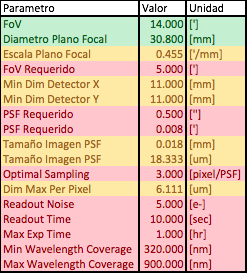
\includegraphics[width=0.5\textwidth]{img/img1}}
  ~ 
  \subfloat[Simbología]{\label{fig:p1_b}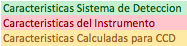
\includegraphics[width=0.3\textwidth]{img/img3}}
  ~ 
  \caption{Tabla de datos y simbología de acuerdo a las especificaciones}
  \label{fig:p1}
\end{figure}



%PREGUNTA 2
\section{Estimar si el diseño óptico es adecuado o es preferible
modificarlo,para el detector seleccionado. En caso de modificación, especifique
los requerimientos para el nuevo diseño óptico.} 

Dado que no existían CCD que
calzaran con las especificaciones, se plantea la siguiente solución:
\begin{itemize}
\item Disminuir escala en el plano focal del instrumento
\end{itemize}

Para ello, se necesita:
\begin{itemize}
\item Disminuir el Field of View
\end{itemize}

Otra opción es aumentar el diámetro, pero como se tiene un gran Field of
View, se descarta esta solución. Luego, se seleccionaron cámaras que
tuvieran el diámetro focal cercano a 30.8. Las mejores cámaras escogidas
fueron:
\begin{itemize}
\item CCD40-42
\item CCD55-30
\end{itemize}

Se elige CCD55-30 y se ajusta Field of View para que cumpla con las
especificaciones de la cámara. De acuerdo a las especificaciones de la cámara,
se recalcula el Field of View para que cumpla los valores tanto de tamaño de los píxeles así
como el tamaño de la cámara, como se puede apreciar en la figura \ref{fig:p2}
\begin{figure}[ht!]
  \centering
  \subfloat[Tabla de datos ajustando especificaciones]{\label{fig:p2_a}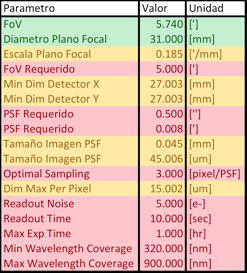
\includegraphics[width=0.5\textwidth]{img/img2}}
  ~ 
  \subfloat[Simbología]{\label{fig:p2_b}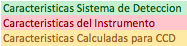
\includegraphics[width=0.3\textwidth]{img/img3}}
  ~ 
  \caption{Tabla de datos ajustada y simbología}
  \label{fig:p2}
\end{figure}

%PREGUNTA 3
\section{Predecir readout noise, dark current y readout time}
Dada las características presentadas en la pregunta 2 (ver figura \ref{fig:p2})
y el datasheet se revisa a continuación readout noise, dark current y readout
frequency:
\subsection{Readout Noise}
A 253[K] dependiendo del amplificador, obtenemos:
\begin{description}
\item [Low Noise Amplifier, A2]: Valor típico: 3 $rms\ [e^-/pixel]$ , valor máximo : 5 $rms\ [e^-/pixel]$
\item [Large Signal Amplifier, A1]: Valor típico: 8 $rms\ [e^-/pixel]$
\end{description}
Podemos trabajar con este detector utilizando Low Noise Amplifier, ya que el
valor máximo es 5 $rms\ [e^-/pixel]$. El valor para A1 (Large Signal Amplifier)
se descarta ya que el valor típico supera lo que se especifica en este trabajo.
Ver además figura \ref{fig:p3_1} para revisar la relación entre readout noise y
frecuencia de lectura.
\begin{figure}[ht!]
  \centering
  \subfloat[Readout Noise v/s Frecuencia]{\label{fig:p3_a}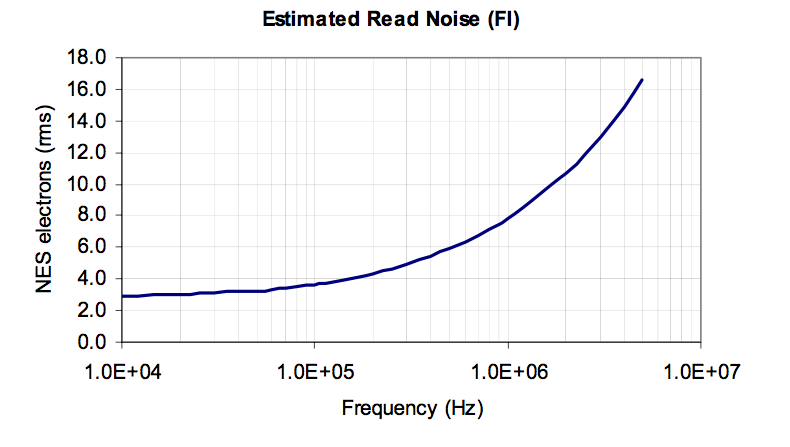
\includegraphics[width=0.8\textwidth]{img/img5}}
  ~ 
  \caption{Readout Noise v/s Frecuencia}
  \label{fig:p3_1}
\end{figure}

\subsection{Dark Current}
Dark Current para este detector, lo podemos ver gráficamente en figura \ref{fig:p3}
\begin{figure}[ht!]
  \centering
  \subfloat[Dark Current v/s Temperatura]{\label{fig:p3_a}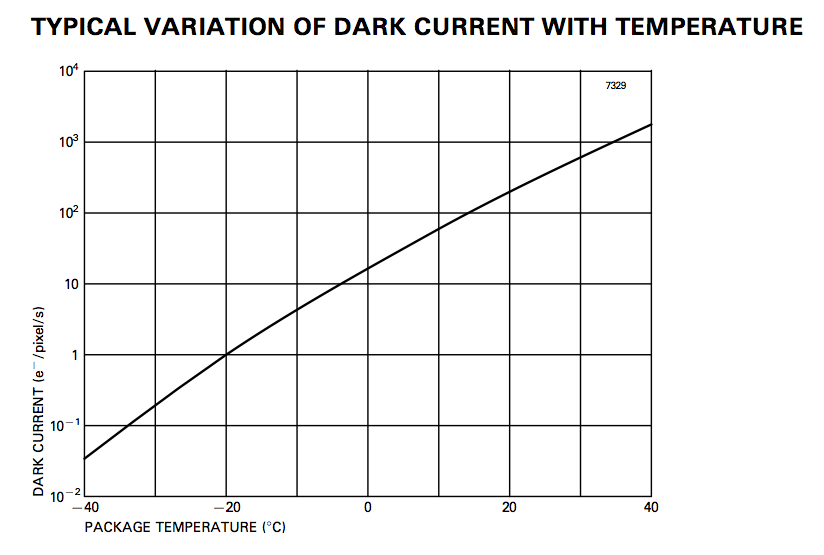
\includegraphics[width=0.8\textwidth]{img/img4}}
  ~ 
  \caption{Variaciones de Dark Current con respecto a la temperatura de Operación}
  \label{fig:p3}
\end{figure}
\subsection{Readout Frequency}
Podemos estimar readout frequency de la siguiente manera:
\begin{description}
\item [pixels]: Número de píxeles total de la cámara
\item [tiempo]: Máximo tiempo de lectura requerido
\item [amplificadores]: Número de amplificadores de salida
\end{description}

Dado los parámetros anteriores el readout frequency se puede calcular: 
\begin{align*}
readout\ frequency &= \frac{pixels}{tiempo*amplificadores}\\
readout\ frequency &= \frac{1252*1152}{10*2} [Hz]\\
readout\ frequency &= 72115.2 [Hz] = 72.1152 [kHz]\\
\end{align*}




%PREGUNTA 4
\section{Estimar los tiempos de exposición para diversos filtros considerando la
eficiencia cuántica del CCD seleccionado y la obtención de una SNR de al menos
10. Analice filtros del tipo SDSS4 (Sloan Digital Sky Survey) para su análisis.}
Para poder analizar esta pregunta es necesario tener en consideracion la figura \ref{fig:p4}

\begin{figure}[ht!]
  \centering
  \subfloat[QE v/s Wavelength]{\label{fig:p4_a}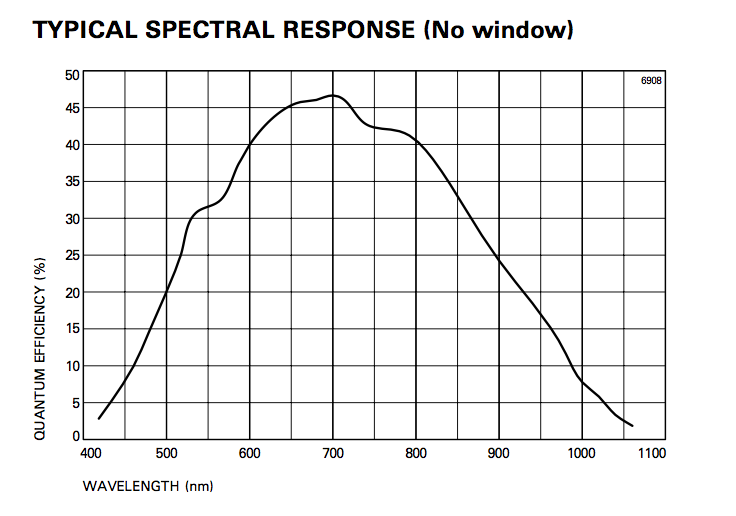
\includegraphics[width=0.8\textwidth]{img/img6}}
  ~ 
  \caption{Quantum Efficiency (\%) v/s Wavelength ($[nm]$)}
  \label{fig:p4}
\end{figure}

%PREGUNTA 5
\section{Especificar los requerimientos de enfriamiento criogénico, en particular
temperatura de operación. Sugerir posibilidades de criogenia.}


\end{document}

